\section{Regularization, bias and variance more in depth}

\subsection{A brief review}
Let's review some useful concepts from the previous sections. \\
Different machine learning techniques with specific sets of hyper-parameters) can represent different types of functions. Generally, a model with more free parameters can approximate a larger number of functions. This ability to represent many functions is referred to as the model \textit{capacity}, which basically represents the model ability to use information effectively. In the context of a Neural Network, adding more neurons (making it wider) or more layers (making it deeper) directly translates to a greater capacity. Remember also that our goal is not simply to fit the training data perfectly, but to ensure that the algorithm works well on unseen data, which means it has to have a good \textit{generalization capability}. if a model has too low of a capacity for the complexity of the data, it will fail to capture the underlying trend, resulting in \textit{underfitting}. Conversely, if the capacity is too high, the model will memorize the noise in the training set rather than the actual signal, leading to \textit{overfitting}. The difference between the training error and the generalization error is known as the \textit{generalization gap}. To achieve good performance on unseen data even when utilizing a high number of parameters, we must rely on \textit{regularization techniques}. The cost function can be modified by introducing a penalty term to limit certain parts of the model-parameter space, or we can use techniques like data augmentation, adding stochastic noise, or applying invariant transformations.

\subsection{Bias vs Variance: a formal derivation for regression}

Generalization and capacity are deeply connected, and finding the right balance is one of the core challenges in Machine Learning. To better understand this kind of tradeoff, we will lay out a formal mathematical demonstration in the case of regression.

Let us consider a training dataset $S = \{x^{(i)}, y^{(i)}\}_{i=1}^n$ such that the true relationship is given by:
\begin{equation}
    y^{(i)} = h^*(x^{(i)}) + \xi^{(i)}
\end{equation}
where $h^*$ is the true underlying function and $\xi^{(i)}$ is an intrinsic noise term drawn from a normal distribution $\mathcal{N}(0, \sigma^2)$. We want to train a regression model, denoted as $\hat{h}_S$, on this dataset $S$.

When we evaluate this model on a new, unseen test sample $(x, y)$ (where $y = h^*(x) + \xi$ with $\xi \in \mathcal{N}(0, \sigma^2)$) we measure the expected test error using the mean squared error:
\begin{equation}
    MSE(x) = \mathbb{E}_{S,\xi}\left[(y - \hat{h}_S(x))^2\right]
\end{equation}
We can decompose this term into \textit{variance} and \textit{bias} by using a known property of expected values: if $A$ and $B$ are two independent real random variables and $\mathbb{E}[A]=0$, then $\mathbb{E}[(A+B)^2] = \mathbb{E}[A^2] + \mathbb{E}[B^2]$. As a corollary, if $B$ is a constant $c$, then $\mathbb{E}[(A+c)^2] = \mathbb{E}[A^2] + c^2$. Applying this claim with $A = \xi$ and $B = h^*(x) - \hat{h}_S(x)$, we obtain:
\begin{equation}
    MSE(x) = \mathbb{E}_{S,\xi}\left[ \left(\xi + (h^*(x) - \hat{h}_S(x))\right)^2 \right] = \mathbb{E}[\xi^2] + \mathbb{E}_S\left[(h^*(x) - \hat{h}_S(x))^2\right]
\end{equation}
Since the expected value of the squared noise $\mathbb{E}[\xi^2]$ is simply its variance $\sigma^2$, the equation simplifies to:
\begin{equation}
    MSE(x) = \sigma^2 + \mathbb{E}_S\left[(h^*(x) - \hat{h}_S(x))^2\right]
\end{equation}
Now, let us define an "average model" $h_{avg}(x) = \mathbb{E}_S[\hat{h}_S(x)]$. This represents an ideal model obtained by drawing an infinite number of datasets, training on all of them, and averaging their predictions (for many cases, it corresponds to one single model trained on infinite samples). By adding and subtracting $h_{avg}(x)$ inside the expectation, we can further decompose the MSE by letting $c = h^*(x) - h_{avg}(x)$ (which is a constant with respect to $S$) and $A = h_{avg}(x) - \hat{h}_S(x)$:
\begin{equation}
    MSE(x) = \sigma^2 + (h^*(x) - h_{avg}(x))^2 + \mathbb{E}_S\left[(h_{avg}(x) - \hat{h}_S(x))^2\right]
\end{equation}
This final equation highlights the three fundamental components of the generalization error:
\begin{equation}
    MSE(x) = \sigma^2 + \text{Bias}^2 + \text{Variance}
\end{equation}
where:
\begin{itemize}
    \item[-] $\sigma^2$ is the irreducible error, caused by the inherent randomness in the dataset.
    \item[-] The \textbf{bias} squared $(h^*(x) - h_{avg}(x))^2$ represents the lack of expressivity of the model. It shows the error introduced because the chosen model cannot represent the true data distribution, not due to a lack of data.
    \item[-] The \textbf{variance} $var(\hat{h}_S(x))$ quantifies how the random nature of the finite dataset introduces error in the model's predictions.
\end{itemize}

\begin{figure}[H]
    \begin{minipage}[c]{0.6\textwidth}
        Bias tends to decrease when the model becomes more complex, while variance shows the opposite behavior, as shown here. As you might imagine is never easy to reach the sweet spot between the two. \\ The concepts of capacity, generalization, bias, and variance are strictly intertwined. A model's capacity dictates its position on the bias-variance tradeoff: low-capacity models lack the expressivity to capture the true function, leading to high bias (underfitting), while high-capacity models tend to memorize the training noise, resulting in high variance (overfitting).
    \end{minipage}\hfill 
    \begin{minipage}[c]{0.39\textwidth}
        \centering
        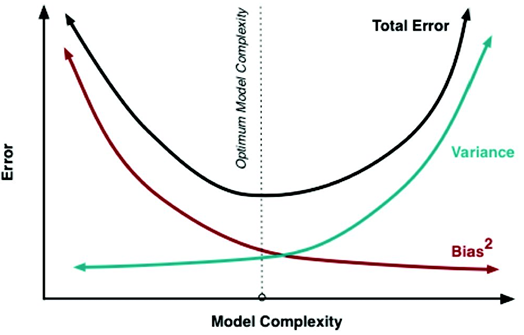
\includegraphics[width=1.0\linewidth]{figuresML/lesson_ml_3_pag_92.png}
    \end{minipage}
\end{figure}
\vspace{-7.5mm}
Since the generalization error (MSE) is the sum of bias squared and variance, achieving good generalization means finding the sweet spot that minimizes both. 

\subsection{Regularization for CNNs}
When dealing with inherently high-capacity models like deep neural networks, regularization acts as a control mechanism: it artificially restricts the model, reducing variance and closing the generalization gap without heavily increasing the bias. In practice, regularization techniques are all based on introducing a "noise" or a confounding factor to our network to prevent it from memorizing the training data. Adding a penalty does this by confounding the loss function, while batch normalization does this by normalizing the inputs on a batch during training.

We have already mentioned the dropout, penalty and batch normalization techniques for regularization. For Convolutional Neural Networks, another incredibly efficient way to regularize the model is \textbf{data augmentation}. By applying various transformations to our data (such as zooming, rotation, elastic deformation, blurring, or adding artificial noise) we artificially expand the training dataset. This forces the network to learn invariant, generalized features rather than memorizing the exact pixel layout of the original input. Here is an example of data augmentation for medical images. 

\begin{center}
    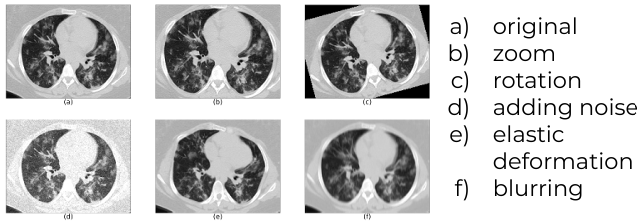
\includegraphics[width=0.5\linewidth]{figuresML/lesson_ml_3_pag_94.png}
\end{center}

Of course, data obtained in such a way will not be independent from the original, and the learning advantages will therefore be limited.

\subsection{Decision trees regularization and Ensembling}
While neural networks are extremely powerful, decision trees remain particularly suited for handling categorical variables and regression problems. However, a standard decision tree is highly prone to overfitting (high variance). To mitigate this, we can apply several regularization constraints:
\begin{itemize}
    \item[-] \textit{Minimum Leaf Size}: Sets the minimum number of samples required to form a terminal node. If too small (e.g., 1), the tree creates very specific, overfitted leaves. Larger values force the tree to be more general.
    \item[-] \textit{Maximum Depth}: Limits the number of levels in the tree. Deep trees capture noise, so setting a limit (e.g., \texttt{max\_depth = 5}) improves generalization.
    \item[-] \textit{Maximum Number of Nodes}: Restricts the total number of internal and leaf nodes, capping overall complexity.
    \item[-] \textit{Minimum Decrease in Loss}: A split is only executed if the improvement in the loss function (e.g., Gini, entropy, MSE) exceeds a certain threshold, preventing useless splits.
    \item[-] \textit{Pruning}: After building a full tree, branches that do not improve performance on a separate validation set are systematically removed.
\end{itemize}

To further combat the high variance inherent in decision trees, we rely on technique called \textbf{ensembling}. \\
Let's take $n$ random variables that are independently and identically distributed with variance $var(x)=\sigma^2$. The variance of their average is $var(\bar{x}) = \frac{\sigma^2}{n}$. If we drop the independence assumption, we introduce a correlation factor $\rho$:
\begin{equation}
    var(\bar{x}) = \rho\sigma^2 + \frac{1-\rho}{n}\sigma^2
\end{equation}
Ensembling is a technique that combines many models called \textit{weak learners} to obtain a more robust metamodel. Here $x_i$ does not represent a training sample, but a different model / decision tree. That's why it is useful to drop the independence assumption, since different models may be trained on the same dataset. By increasing the number of models $n$ and decreasing the correlation $\rho$ between them, the overall variance drops significantly. There are four main ways to do this: using different algorithms, using different training sets, implementing bagging or implementing boosting. Let's see how those work

\textbf{Bagging} or \textbf{Bootstrap Aggregating)} is a typical method used in statistics to measure uncertainty. To implement it we define bootstrap samples $Z \sim S$ (where $S$ is our original training sample), sampling $M$ times from the training set \textit{with replacement} (each subsample has the same dimension as the initial dataset but with duplicates and missing data). We train a single model $G_m$ on each bootstrap sample, and we define the metamodel by averaging their outputs:
\begin{equation*}
   G(m) = \frac{\sum_{m=1}^M G_m(x)}{M}
\end{equation*}
The larger $M$ is, the smaller the variance. \newline\newline
This technique is fundamental for the so called \textit{Random Forest} algorithms. Bagging is well suited for decision trees because they inherently have high variance. However, to reduce correlation among single decision trees, random forests perform bagging plus a random subsampling in the feature space. This decreases the correlation term $\rho$.

Unlike bagging, where models are trained independently, \textbf{boosting} trains models sequentially. The logic follows a recursive pattern:
\begin{enumerate}
    \item We make the first split.
    \item We identify the mistakes made by the current model.
    \item We increase the weight of those misclassified samples.
    \item Now the new weak learner may choose another decision boundary focusing on the hardest samples.
    \item We apply this recursively.
\end{enumerate}
This logic is the foundation of algorithms like AdaBoost (applying weights to the hardest samples) or Gradient Boosting/XGBoost (finding the minimum of the residual error).


\subsection{More on optimizers}
The core of the learning process is the optimization of the cost function $J(\theta)$. We already saw the stochastic gradient descent and mini-batch stochastic gradient descent methods for optimization, which update the parameters $\theta_i$ of the algorithm as follows:
\begin{equation}
    \theta_j:=\theta_j - \alpha \dfrac{\partial J(\theta_j)}{\partial\theta_j}
\end{equation}
where $\alpha$ is the learning rate and $J(\theta_j)$ is the cost function.
However, to improve convergence, several advanced optimizers modify this basic update rule. Let's take a look at some of them.

\textbf{SGD with Momentum}:
We modify the parameter update by inserting a new parameter called "velocity" $v_t$, which accumulates past gradients:
\begin{equation}
\begin{aligned}
    v_t &= \beta v_{t-1} + \frac{\partial J(\theta_j)}{\partial \theta_j} \\
    \theta_j &:= \theta_j - \alpha \left( \beta v_{t-1} + \frac{\partial J(\theta_j)}{\partial \theta_j} \right)
\end{aligned}
\end{equation}
The momentum coefficient $\beta$ (typically around 0.9) regulates how much past information is retained. This alleviates the problem of SGD stopping at local optima and reduces oscillations. However, if the local valleys are deep and momentum is exhausted, it can still get trapped in a local minimum.

\textbf{AdaGrad}:
AdaGrad provides an adaptive learning rate by tracking the sum of the squared gradients, $r_j^{(t)}$:
\begin{equation}
    r_j^{(t)} = r_j^{(t-1)} + \left(\frac{\partial J(\theta_j)}{\partial \theta_j}\right)^2 \quad \Longrightarrow \quad \theta_j := \theta_j - \frac{\alpha}{\sqrt{r_j^{(t)}} + \epsilon} \frac{\partial J(\theta_j)}{\partial \theta_j}
\end{equation}
If a parameter has been strongly updated in the past, it will be updated a little less in the future. This works well with sparse data distributions, but in later stages, the sum of square gradients in the denominator becomes very large, causing the parameter update to approach zero prematurely.

\textbf{RMSprop}:
RMSprop fixes AdaGrad's vanishing learning rate by replacing the accumulator with an exponential moving average:
\begin{equation}
    r_j^{(t)} = \beta r_j^{(t-1)} + (1-\beta)\left(\frac{\partial J(\theta_j)}{\partial \theta_j}\right)^2
\end{equation}
By progressively "forgetting" older gradients (regulated by the decay coefficient $\beta$), RMSprop avoids the continuous accumulation of the second momentum. It works incredibly well, though it can be unstable in the very early stages of optimization.

\textbf{Adam (Adaptive Moment Estimation)}:
Adam delightfully merges momentum and RMSprop by keeping track of both the first momentum and the second momentum, adding a correction for initialization bias:
\begin{align}
    m_t &= \beta_1 m_{t-1} + (1-\beta_1)\frac{\partial J(\theta_j)}{\partial \theta_j} \\
    v_t &= \beta_2 v_{t-1} + (1-\beta_2)\left(\frac{\partial J(\theta_j)}{\partial \theta_j}\right)^2
\end{align}
Bias corrections:
\begin{equation}
    \hat{m}_t = \frac{m_t}{1-\beta_1^t} \quad \text{and} \quad \hat{v}_t = \frac{v_t}{1-\beta_2^t}
\end{equation}
Final update:
\begin{equation}
    \theta_j := \theta_j - \alpha \frac{\hat{m}_t}{\sqrt{\hat{v}_t} + \epsilon}
\end{equation}
Typically, hyperparameters are set to $\beta_1 = 0.9$, $\beta_2 = 0.999$, and $\epsilon = 10^{-8}$.
